%%%%%%%%%%%%%%%%%%%%%%%%%%%%%%%%%%%%%%%%%
% Beamer Presentation
% LaTeX Template
% Version 1.0 (10/11/12)
%
% This template has been downloaded from:
% http://www.LaTeXTemplates.com
%
% License:
% CC BY-NC-SA 3.0 (http://creativecommons.org/licenses/by-nc-sa/3.0/)
%
%%%%%%%%%%%%%%%%%%%%%%%%%%%%%%%%%%%%%%%%%

%----------------------------------------------------------------------------------------
%	PACKAGES AND THEMES
%----------------------------------------------------------------------------------------

\documentclass{beamer}
\usepackage[spanish]{babel}
\usepackage[utf8]{inputenc}
\mode<presentation> {

% The Beamer class comes with a number of default slide themes
% which change the colors and layouts of slides. Below this is a list
% of all the themes, uncomment each in turn to see what they look like.

%\usetheme{default}
%\usetheme{AnnArbor}
%\usetheme{Antibes}
%\usetheme{Bergen}
%\usetheme{Berkeley}
%\usetheme{Berlin}
%\usetheme{Boadilla}
%\usetheme{CambridgeUS}
%\usetheme{Copenhagen}
%\usetheme{Darmstadt}
%\usetheme{Dresden}
%\usetheme{Frankfurt}
%\usetheme{Goettingen}
%\usetheme{Hannover}
%\usetheme{Ilmenau}
%\usetheme{JuanLesPins}
%\usetheme{Luebeck}
%\usetheme{Madrid}
%\usetheme{Malmoe}
%\usetheme{Marburg}
%\usetheme{Montpellier}
\usetheme{PaloAlto}
%\usetheme{Pittsburgh}
%\usetheme{Rochester}
%\usetheme{Singapore}
%\usetheme{Szeged}
%\usetheme{Warsaw}

% As well as themes, the Beamer class has a number of color themes
% for any slide theme. Uncomment each of these in turn to see how it
% changes the colors of your current slide theme.

%\usecolortheme{albatross}
%\usecolortheme{beaver}
%\usecolortheme{beetle}
%\usecolortheme{crane}
%\usecolortheme{dolphin}
%\usecolortheme{dove}
%\usecolortheme{fly}
%\usecolortheme{lily}
%\usecolortheme{orchid}
%\usecolortheme{rose}
%\usecolortheme{seagull}
%\usecolortheme{seahorse}
%\usecolortheme{whale}
%\usecolortheme{wolverine}

%\setbeamertemplate{footline} % To remove the footer line in all slides uncomment this line
%\setbeamertemplate{footline}[page number] % To replace the footer line in all slides with a simple slide count uncomment this line

%\setbeamertemplate{navigation symbols}{} % To remove the navigation symbols from the bottom of all slides uncomment this line
}

\usepackage{graphicx} % Allows including images
\usepackage{booktabs} % Allows the use of \toprule, \midrule and \bottomrule in tables

%----------------------------------------------------------------------------------------
%	TITLE PAGE
%----------------------------------------------------------------------------------------

\title[Práctica 1]{Práctica 1: Eficiencia} % The short title appears at the bottom of every slide, the full title is only on the title page

\author{Algorítmica} % Your name
\institute[UGR] % Your institution as it will appear on the bottom of every slide, may be shorthand to save space
{
Universidad de Granada \\ % Your institution for the title page
\medskip

}
\date{\today} % Date, can be changed to a custom date

\begin{document}

\begin{frame}
\titlepage % Print the title page as the first slide
\end{frame}

\begin{frame}
\frametitle{Indice} % Table of contents slide, comment this block out to remove it
\tableofcontents % Throughout your presentation, if you choose to use \section{} and \subsection{} commands, these will automatically be printed on this slide as an overview of your presentation
\end{frame}

%----------------------------------------------------------------------------------------
%	PRESENTATION SLIDES
%----------------------------------------------------------------------------------------

\section{Introducción }
\begin{frame}
	\frametitle{Introducción}
	\begin{itemize}
		\item El objetivo de ésta práctica es analizar eficiencias de forma empírica e híbrida.
		\item Para ello, hemos recogido los diferentes tiempos de los diferentes algoritmos que se ofrecían y los hemos comparado.
		\item En nuestro caso concreto, hemos utilizado la biblioteca de C++ más moderna y precisa destinado a obtener tiempos de reloj: la biblioteca \textbf{chrono}
		\end{itemize}
\end{frame}
\begin{frame}
	\frametitle{Especificaciones de la máquina}
	\begin{itemize}
		
		\item Procesador: Intel Core i5-3337U (2.7GHz x 2)
		\item Memoria RAM: 4GB
	    \item Disco Duro: 500GB 5400 rpm
		\item SO: Manjaro Linux 15.2 Capella 64 bits
	\end{itemize}
	
\end{frame}


%------------------------------------------------
\section{Ordenación} % Sections can be created in order to organize your presentation into discrete blocks, all sections and subsections are automatically printed in the table of contents as an overview of the talk
%------------------------------------------------
\begin{frame}
	\frametitle{Ordenación}
	Según hemos ido hemos estudiado, estos algoritmos que presentamos tienen teóricamente y calculando a partir del código una eficiencia de $O(n^2 )$. Como esto es teórico, vamos a ver si efectivamente (o no) los algoritmos proporcionados se parecen a la gráfica de $n^2$ recogiendo la información de 99 posibilidades distintas en cada algoritmo.
	\begin{figure}
		\centering
		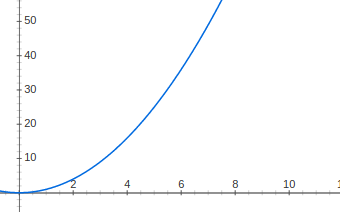
\includegraphics[width=0.5\linewidth]{imagenes/enecuadrado.png}
		\caption{Gráfica de la función $n^2$}
		\label{fig:E1}
	\end{figure}

\end{frame}

\subsection{Burbuja}
\begin{frame}
	\frametitle{Burbuja}
	La gráfica empírica obtenida ha sido:
	\begin{figure}
		\centering
		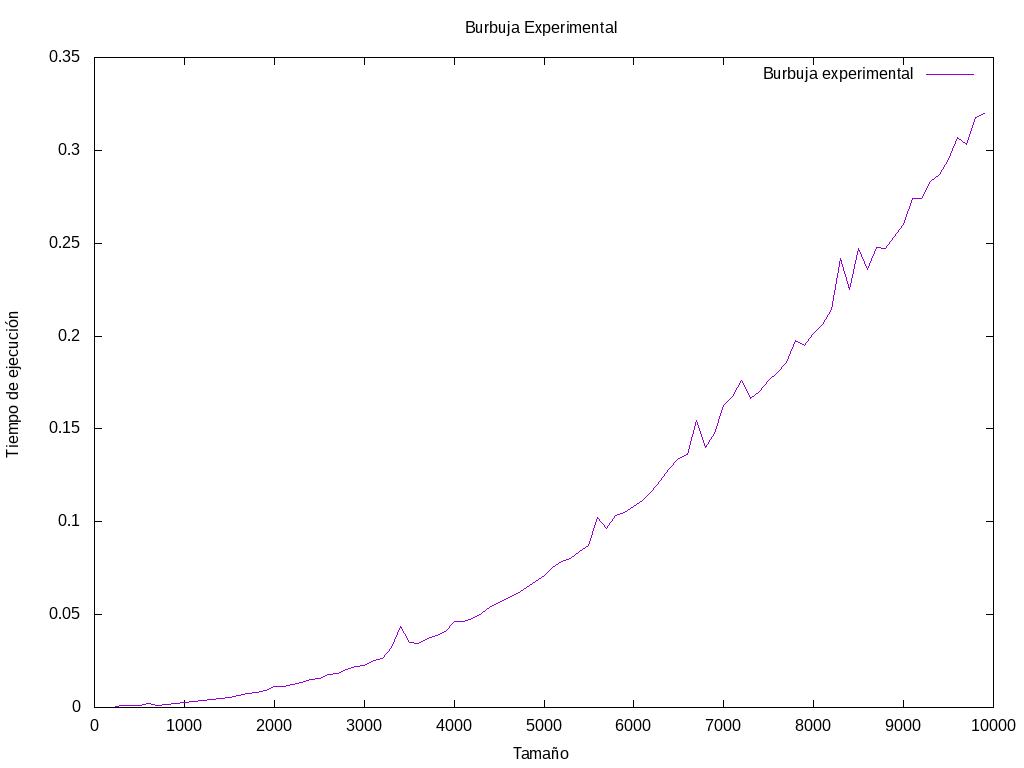
\includegraphics[width=0.7\linewidth]{imagenes/burbuja-experimental.png}
		\caption{Algoritmo de Burbuja, gráfica empírica.}
		\label{fig:E2}
	\end{figure}
	
\end{frame}

\begin{frame}
	\frametitle{Burbuja}
	La gráfica híbrida obtenida ha sido:
	\begin{figure}
		\centering
		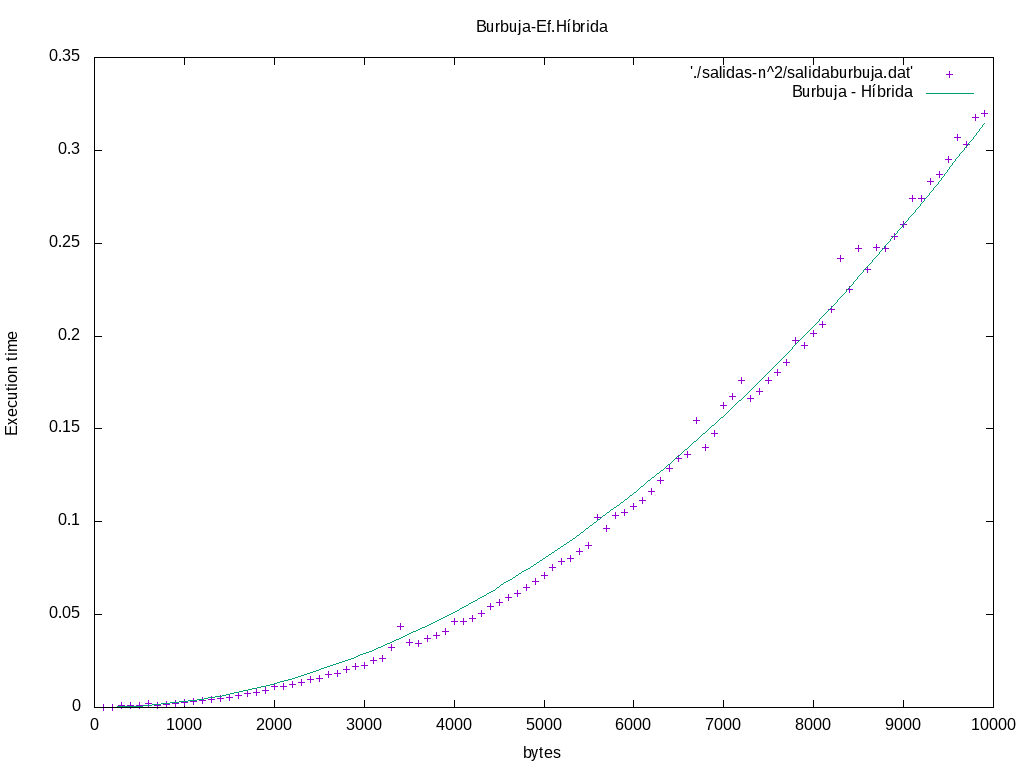
\includegraphics[width=0.7\linewidth]{imagenes/burbuja-hibrida.png}
		\caption{Ajuste híbrido algoritmo Burbuja y función $n^2$}
		\label{fig:E3}
	\end{figure}	
\end{frame}





\subsection{Selección}
\begin{frame}
	\frametitle{Selección}
	La gráfica empírica obtenida ha sido:
	\begin{figure}
		\centering
		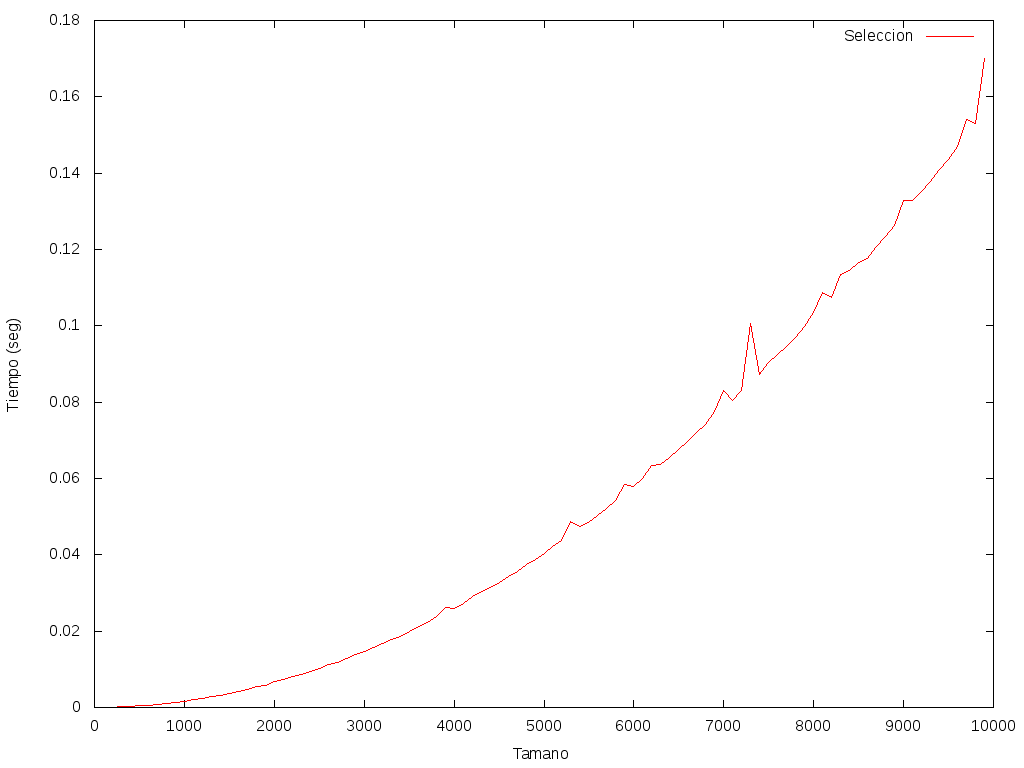
\includegraphics[width=0.7\linewidth]{imagenes/seleccionLines.png}
		\caption{Algoritmo de selección, gráfica empírica. }
		\label{fig:E4}
	\end{figure}
	
\end{frame}

\begin{frame}
	\frametitle{Selección}
	La gráfica híbrida obtenida ha sido:
	\begin{figure}
		\centering
		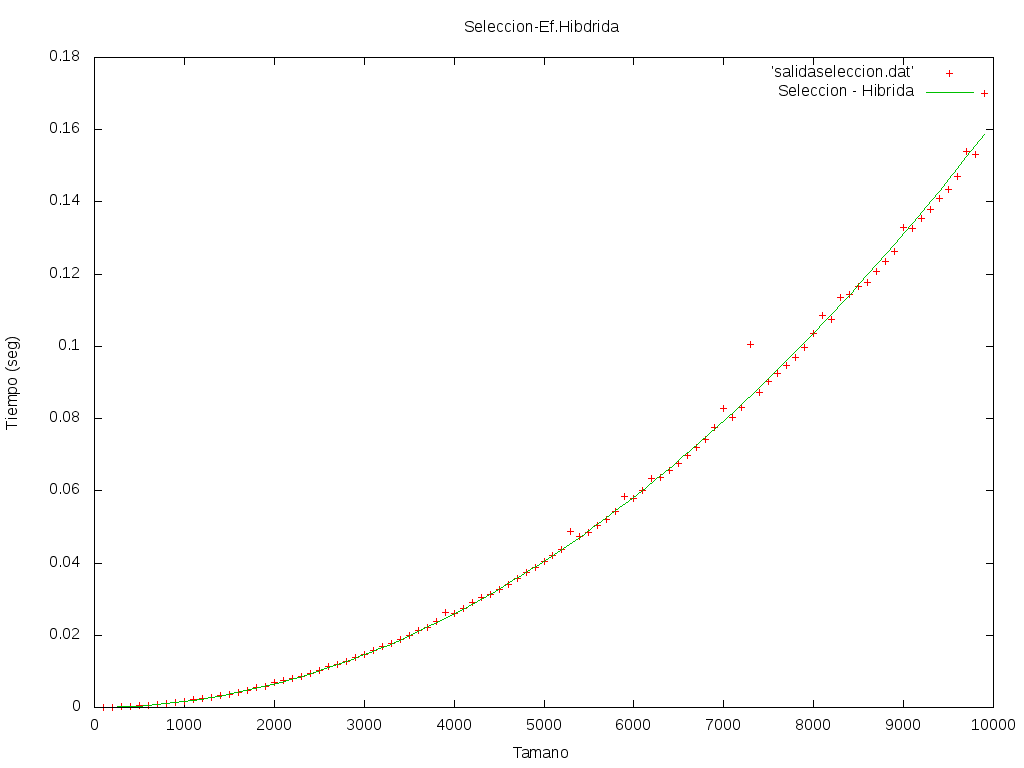
\includegraphics[width=0.7\linewidth]{imagenes/seleccion-hibrida.png}
		\caption{Gráfica ajuste híbrido. Selección y $n^2$}
		\label{fig:E5}
	\end{figure}
	
\end{frame}
\subsection{Inserción}
\begin{frame}
	\frametitle{Inserción}
	La gráfica empírica obtenida ha sido:
	\begin{figure}
		\centering
		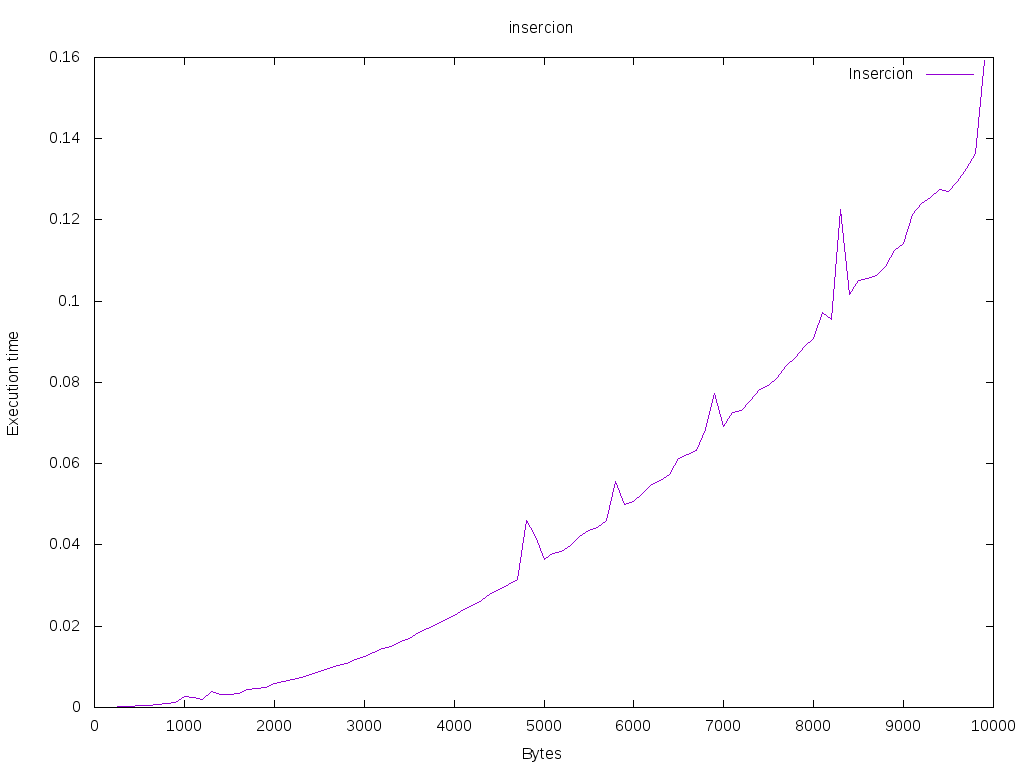
\includegraphics[width=0.7\linewidth]{imagenes/insercion.png}
		\caption{Algoritmo de Inserción, gráfica empírica.}
		\label{fig:E6}
	\end{figure}
	
\end{frame}

\begin{frame}
	\frametitle{Inserción}
	La gráfica híbrida obtenida ha sido:
	\begin{figure}
		\centering
		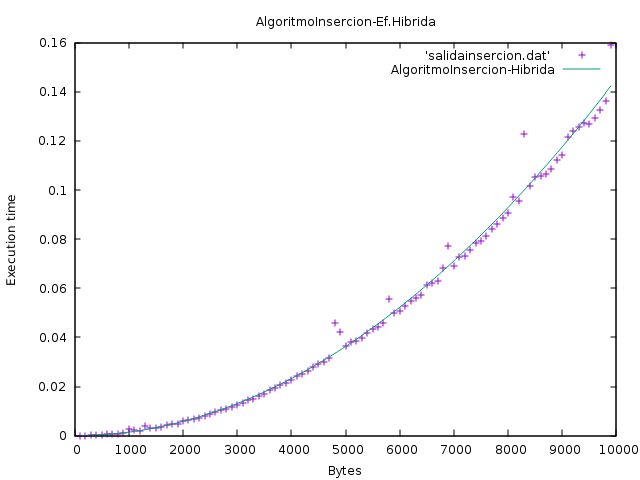
\includegraphics[width=0.7\linewidth]{imagenes/algoritmoInsercion-hibrida}
		\caption{Gráfica ajuste híbrido. Inserción y $n^2$}
		\label{fig:E7}
	\end{figure}
	
\end{frame}


\begin{frame}
	\frametitle{Algoritmos $n^2$}
	Por último, mostramos el porcentaje de error así como las constantes ocultas obtenidas.\\
	
	\begin{center}
		\begin{tabular}{| l | c | r |}
			\hline
			\textbf{Algoritmo} & \textbf{Constante Oculta} & \textbf{Error} \\ \hline
			Burbuja & a0 = 3.20873e-09 & +/- 1.403e-11 (0.4372\%)\\ \hline
			Selección & a0 = 1.61988e-09 & +/- 4.818e-12 (0.2975\%) \\ \hline
			Inserción & a0 = 1.45151e-09 &  +/- 8.337e-12    (0.5743\%) \\ \hline
		\end{tabular}
	\end{center}

	
	
\end{frame}


\section{Ordenación rápida} % Sections can be crea es muy bajoted in order to organize your presentation into discrete blocks, all sections and subsections are automatically printed in the table of contents as an overview of the talk
%------------------------------------------------
\begin{frame}
	\frametitle{Ordenación rápida}
	Según hemos ido estudiado, estos algoritmos que presentamos tienen teóricamente y calculando a partir del código una eficiencia de $O(n*\log(n) )$. Como esto es teórico, vamos a ver si efectivamente (o no) los algoritmos proporcionados se parecen a la gráfica de $n*\log(n)$ recogiendo la información de 99 posibilidades distintas en cada algoritmo.
	\begin{figure} [H]
		\centering
		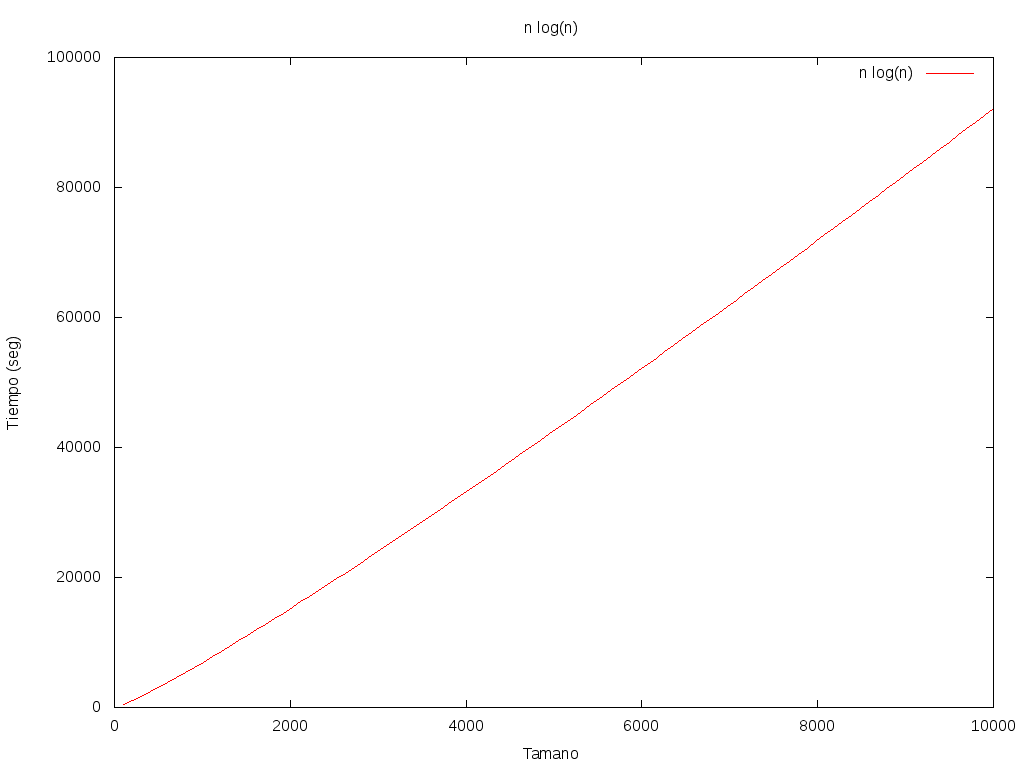
\includegraphics[width=0.5\linewidth]{imagenes/nlog(n)3.png}
		\caption{Gráfica de la función $n*log(n)$}
		\label{fig:E8}
	\end{figure}
	
\end{frame}
\subsection{Quick Sort}
\begin{frame}
	\frametitle{Quick Sort}
	La gráfica empírica obtenida ha sido:
	\begin{figure}
		\centering
		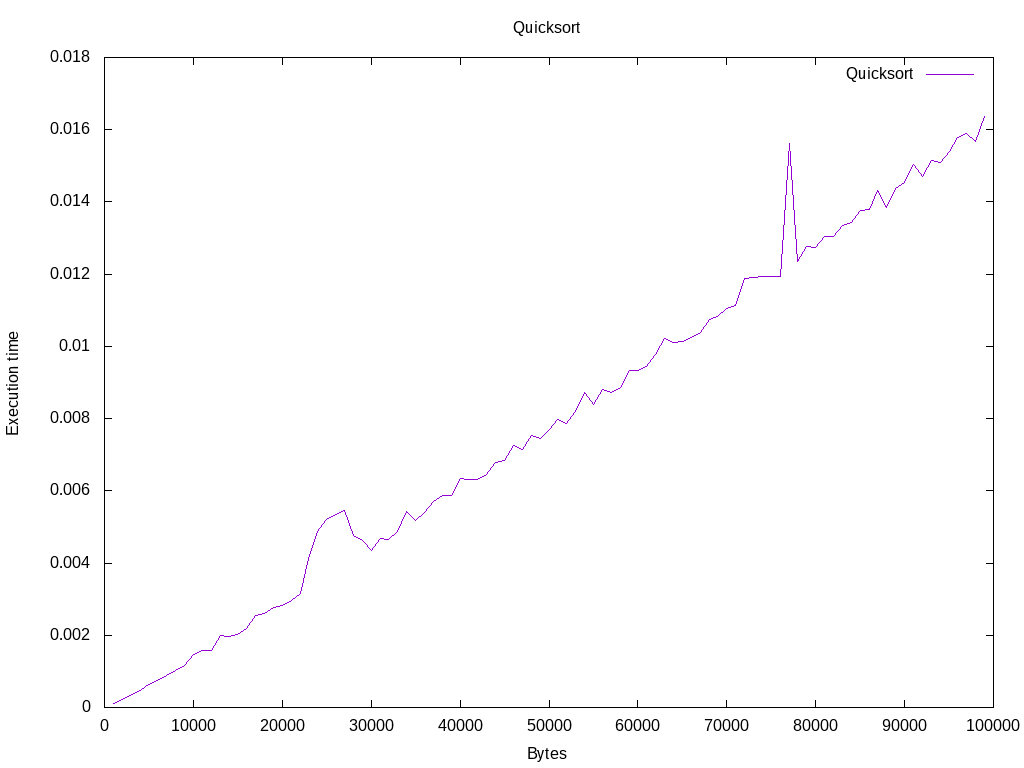
\includegraphics[width=0.7\linewidth]{imagenes/quicksort.png}
		\caption{Algoritmo Quicksort, gráfica empírica. }
		\label{fig:E9}
	\end{figure}
	
\end{frame}

\begin{frame}
	\frametitle{Quick Sort}
	La gráfica híbrida obtenida ha sido:
	\begin{figure}
		\centering
		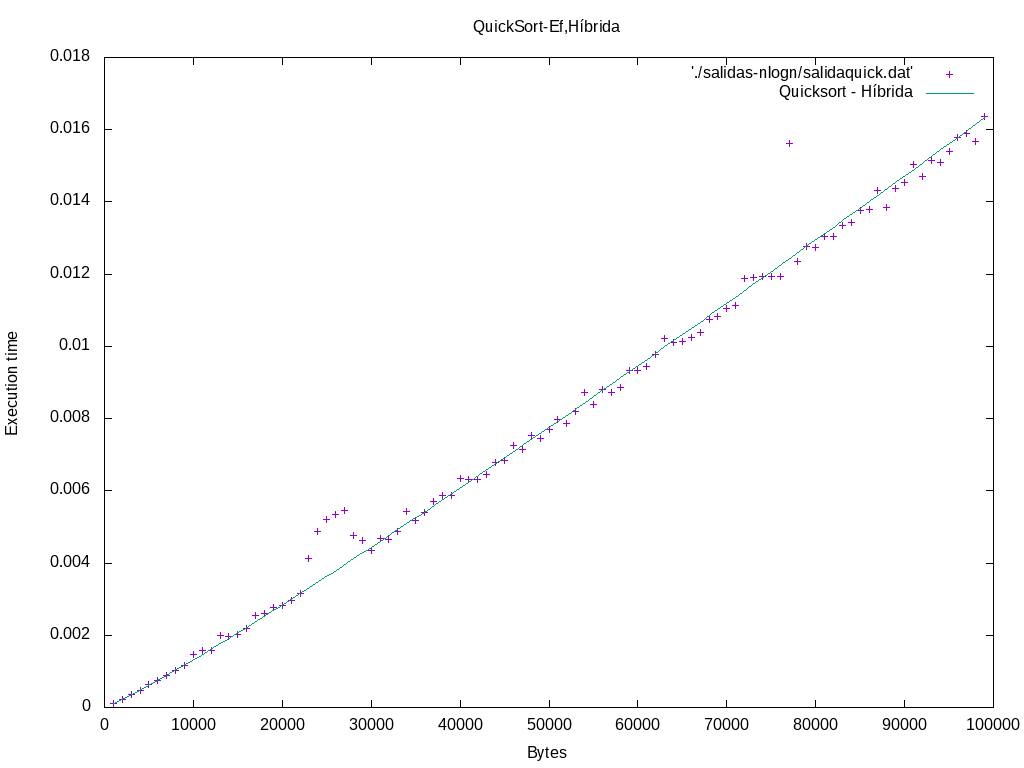
\includegraphics[width=0.7\linewidth]{imagenes/quicksort-hibrida.png}
		\caption{Gráfica híbrida Quicksort.}
		\label{fig:E10}
	\end{figure}
\end{frame}
\subsection{Heap Sort}
\begin{frame}
	\frametitle{Heap Sort}
	La gráfica empírica obtenida ha sido:
	\begin{figure}
		\centering
		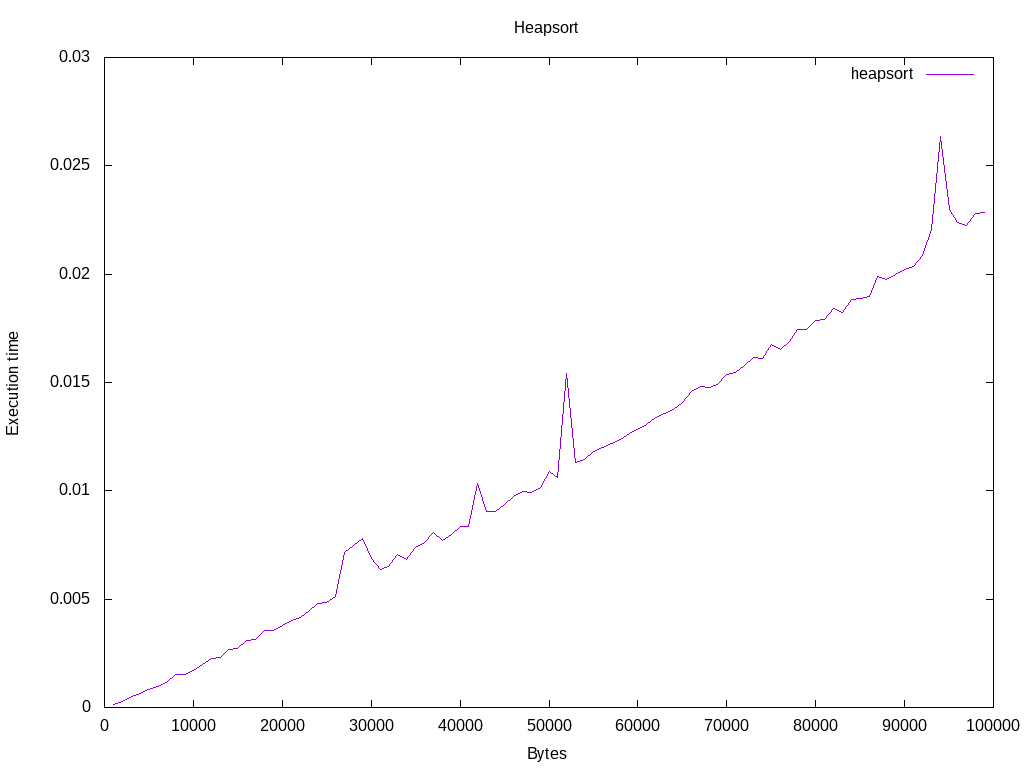
\includegraphics[width=0.7\linewidth]{imagenes/heapsort.png}
		\caption{Heapsort, gráfica empírica.}
		\label{fig:E11}
	\end{figure}
	
\end{frame}

\begin{frame}
	\frametitle{Heap Sort}
	La gráfica híbrida obtenida ha sido:
	\begin{figure}
		\centering
		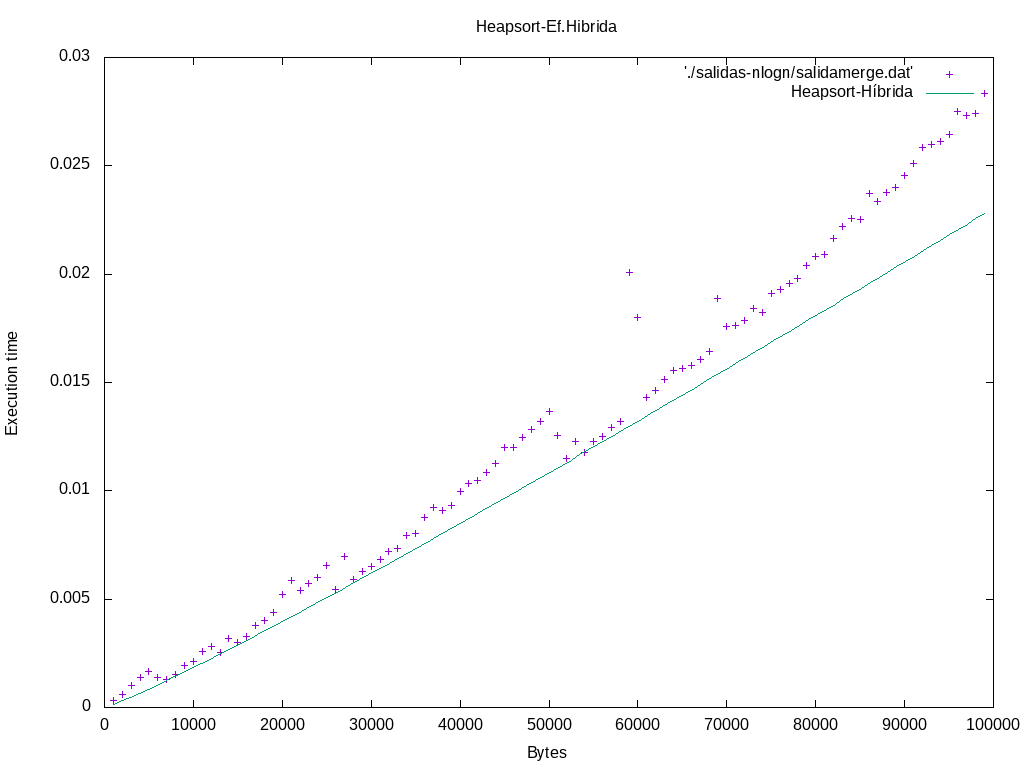
\includegraphics[width=0.7\linewidth]{imagenes/heapsort-hibrida.png}
		\caption{Heapsort, gráfica híbrida.}
		\label{fig:E12}
	\end{figure}
\end{frame}

\begin{frame}
	\frametitle{Heap Sort}
	Este algoritmo lo hemos ejecutado en otra máquina más potente, de esta manera, podemos ver como varían los tiempos de ejecución del mismo algoritmo, ejecutado en dos máquinas distintas.
	\begin{itemize}
		\item Procesador (frecuencia): Intel Core i7-5500U (3.0 GHz x 2)
		\item Memoria RAM: 4 GB
		\item Disco duro: SSD 256 GB
		\item S.O: Linux Mint 17.3 Cinnamon 64-bit
	\end{itemize}
\end{frame}

\begin{frame}
	\frametitle{Heap Sort}
	El ajuste de ambas gráficas es el siguiente:
	\begin{figure}
		\centering
		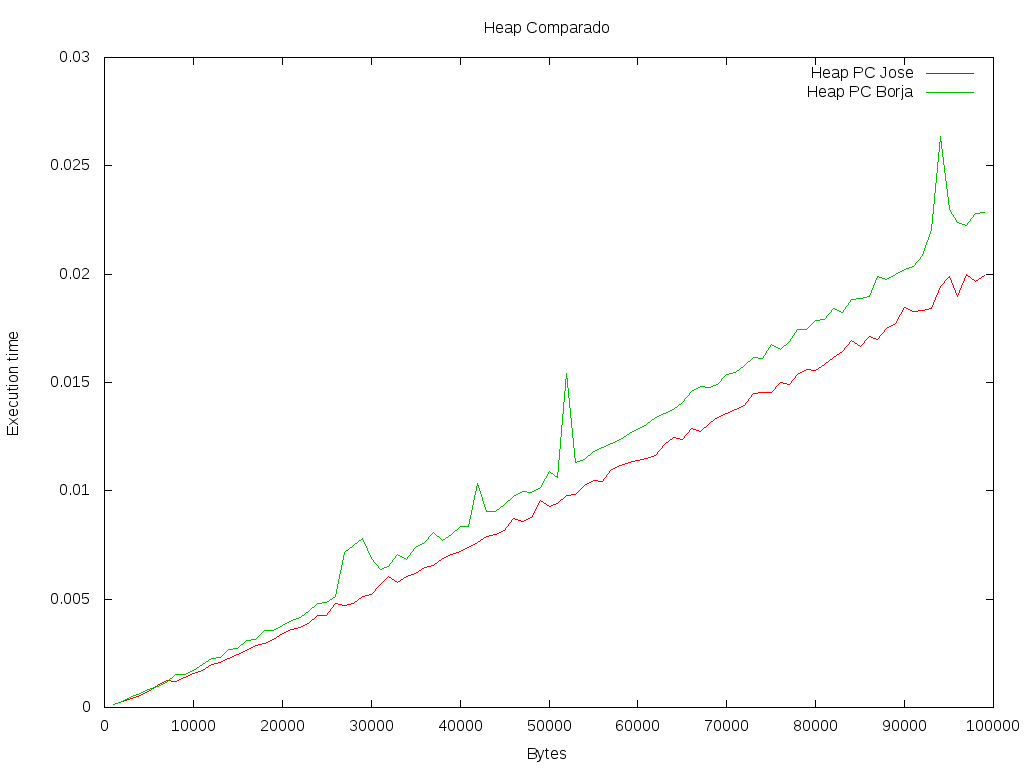
\includegraphics[width=0.7\linewidth]{imagenes/HeapComparado.png}
		\caption{Comparación en dos máquinas. Heapsort.}
		\label{fig:E13}
	\end{figure}
\end{frame}
\subsection{Merge Sort}
\begin{frame}
	\frametitle{Merge Sort}
	La gráfica empírica obtenida ha sido:
	\begin{figure}
		\centering
		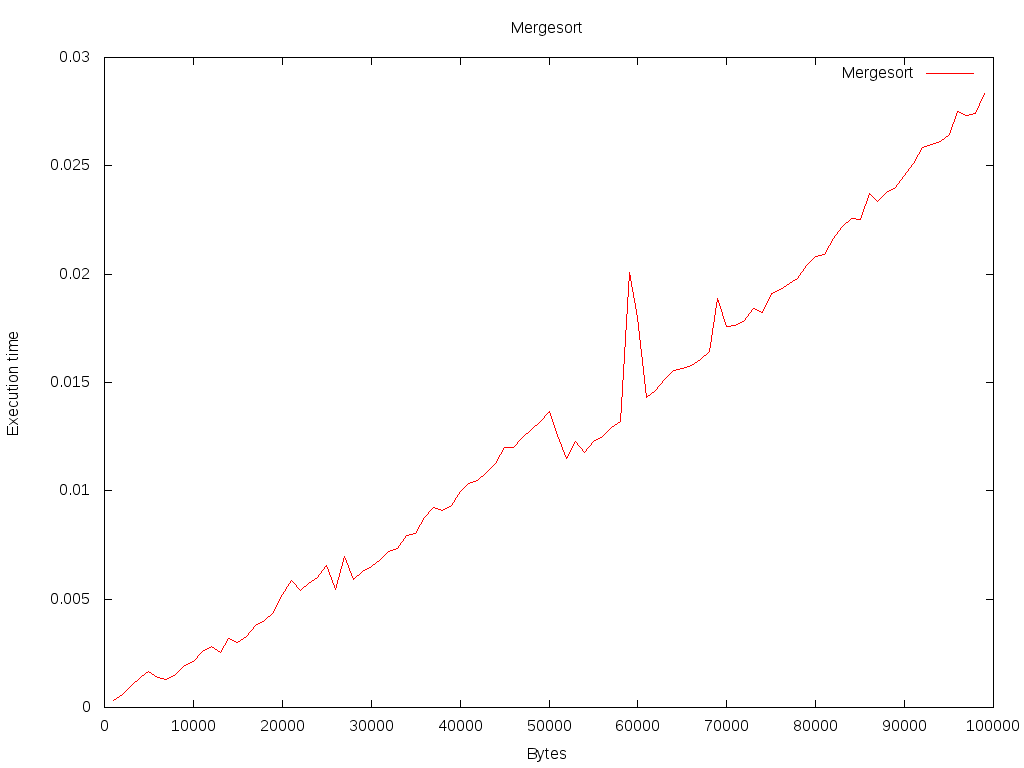
\includegraphics[width=0.7\linewidth]{imagenes/mergesort.png}
		\caption{Mergesort, gráfica empírica.}
		\label{fig:E14}
	\end{figure}
	
\end{frame}

\begin{frame}
	\frametitle{Merge Sort}
	La gráfica híbrida obtenida ha sido:
	\begin{figure}
		\centering
		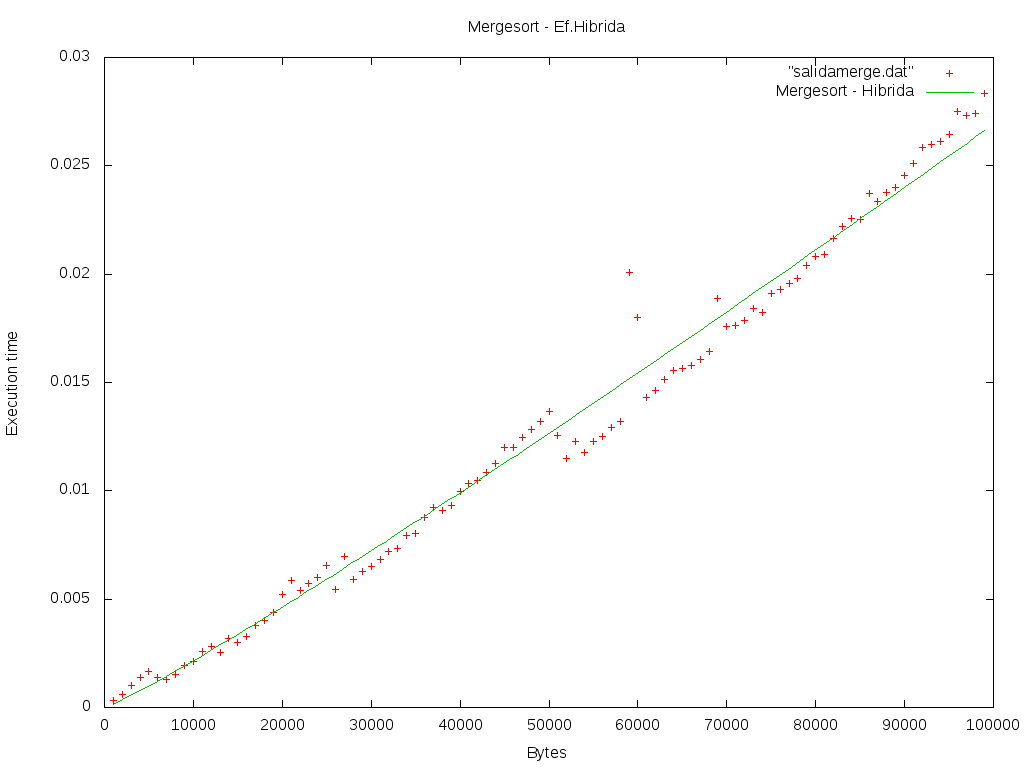
\includegraphics[width=0.7\linewidth]{imagenes/mergesort-hibrida.png}
		\caption{Mergesort, gráfica híbrida.}
		\label{fig:E15}
	\end{figure}
\end{frame}

\begin{frame}
	\frametitle{Algoritmos $n*log(n)$}
	Por último, mostramos el porcentaje de error así como las constantes ocultas.\\
	
	\begin{center}
		\begin{tabular}{| l | c | r |}
			\hline
			\textbf{Algoritmo} & \textbf{Constante Oculta} & \textbf{Error} \\ \hline
			Mergesort & a0 = 2.33821e-08 & +/- 1.564e-10 (0.6689\%)\\ \hline
			Quicksort & a0 = 1.43368e-08 & +/- 7.621e-11 (0.5315\%) \\ \hline
			Heapsort & a0 = 2.00227e-08 & +/- 1.222e-10    (0.6104\%) \\ \hline
		\end{tabular}
	\end{center}

	
	
\end{frame}

\section{Floyd}
\begin{frame}
	\frametitle{Floyd}
	El algoritmo de Floyd, a diferencia de los anteriores, no es un algoritmo de ordenación. Su función, es la de encontrar el camino mínimo en grafos. La eficiencia teórica de este algoritmo es $O(n^3)$. Además de analizar la eficiencia empírica e híbrida, hemos realizado un ajuste erróneo, para demostrar que efectivamente la eficiencia de este algoritmo es la anteriormente mencionada.
\end{frame}

\begin{frame}
	\frametitle{Floyd}
	La gráfica empírica obtenida ha sido:
	\begin{figure}
		\centering
		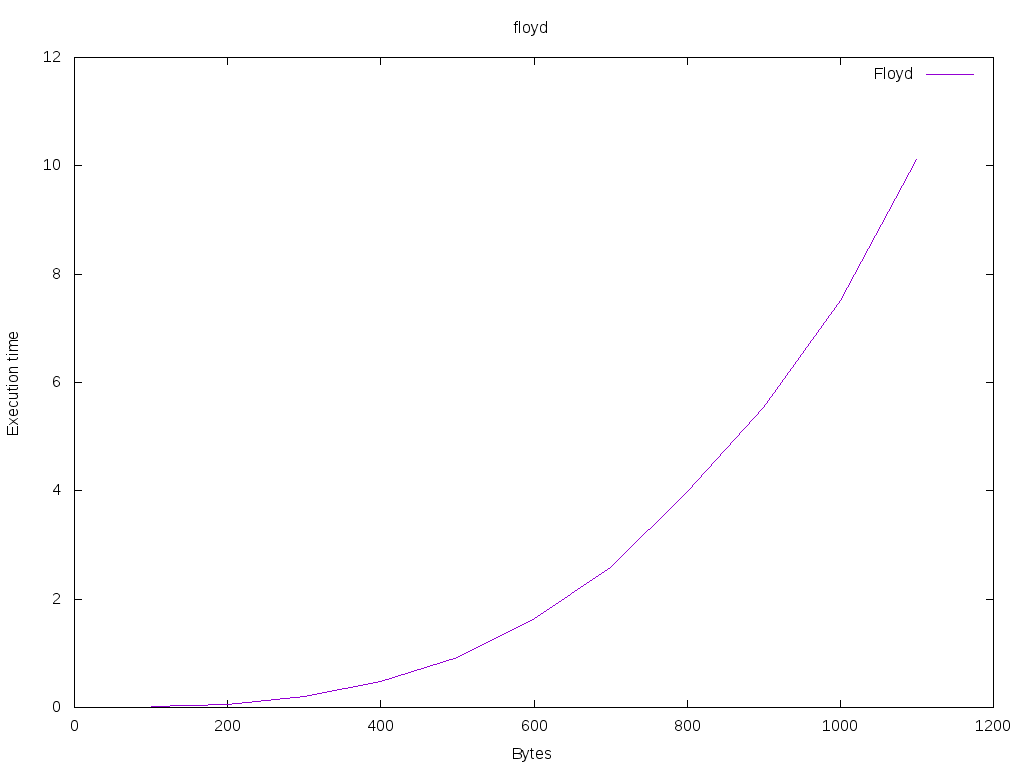
\includegraphics[width=0.7\linewidth]{imagenes/floyd.png}
		\caption{Floyd, gráfica empírica.}
		\label{fig:E16}
	\end{figure}
	
\end{frame}

\begin{frame}
	\frametitle{Floyd}
	La gráfica híbrida obtenida ha sido:
	\begin{figure}
		\centering
		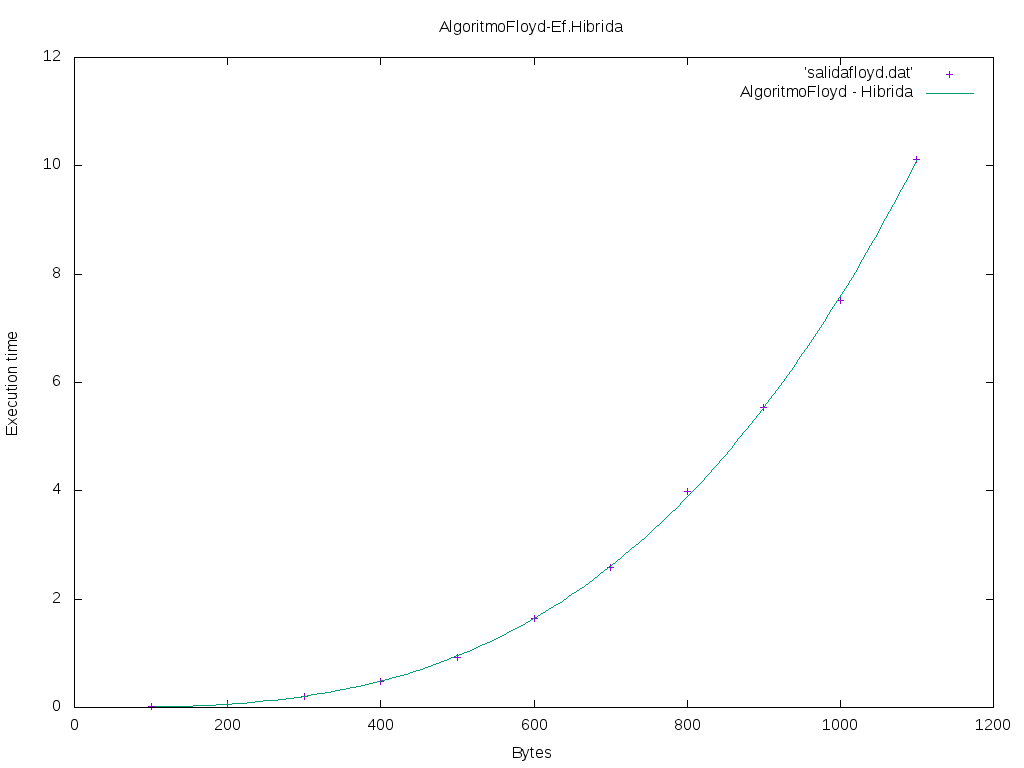
\includegraphics[width=0.7\linewidth]{imagenes/algoritmoFloyd-hibrida.png}
		\caption{Floyd, gráfica híbrida.}
		\label{fig:E17}
	\end{figure}
\end{frame}

\begin{frame}
	\frametitle{Floyd}
	Ajuste híbrido erróneo ($O(n^3)$ ajustada a una función $O(n * log(n))$.
	\begin{figure}
		\centering
		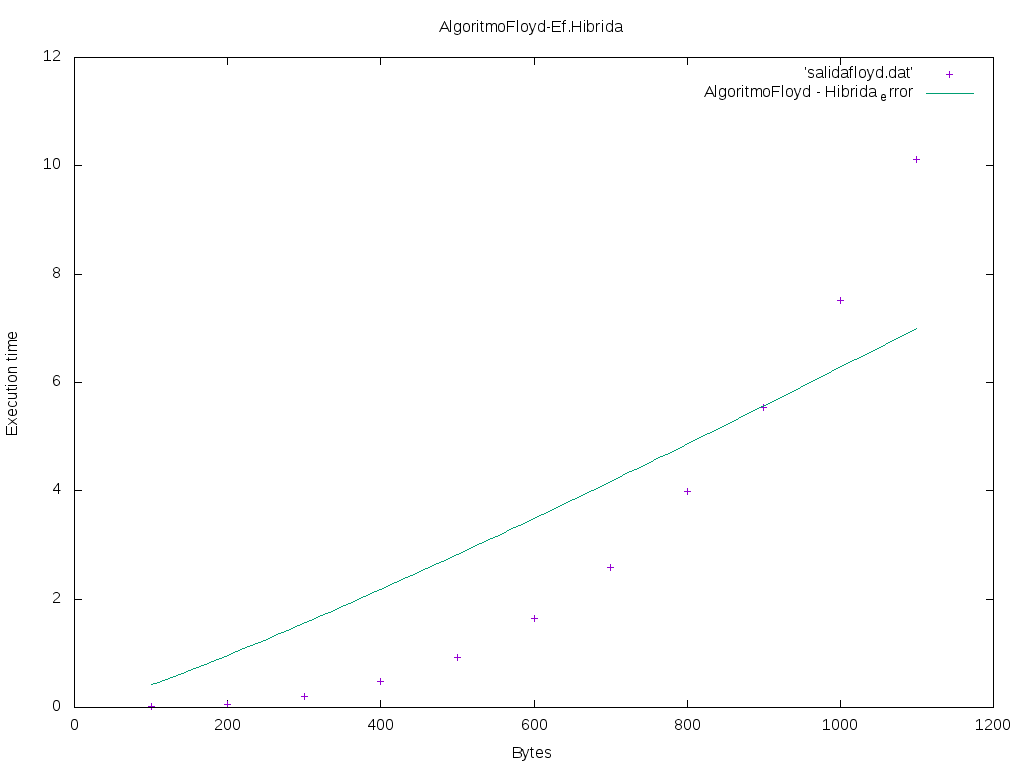
\includegraphics[width=0.7\linewidth]{imagenes/FloydError.png}
		\caption{Floyd, ajuste erróneo.}
		\label{fig:E18}
	\end{figure}
\end{frame}

\begin{frame}
	\frametitle{Floyd $O(n^3)$}
	Por último, mostramos el porcentaje de error así como las constantes ocultas de ambos ajustes.\\
	
	\begin{center}
		\begin{tabular}{| l | c | r |}
			\hline
			\textbf{Algoritmo} & \textbf{Constante Oculta} & \textbf{Error} \\ \hline
			Floyd & a0 = 7.59068e-09 & +/- 2.163e-11    (0.2849\%)\\ \hline
			Floyd erróneo & a0 = 0.000908818 & +/- 0.0001093 (12.03\%) \\ \hline
		\end{tabular}
	\end{center}

\end{frame}

\section{Hanoi}

\begin{frame}
	\frametitle{Hanoi}
	El algoritmo de Hanoi, se encarga específicamente de resolver el problema de las torres de Hanoi. Este algoritmo presenta una eficiencia teórica de $O(2^n)$, lo que hace que el número de entradas para este algoritmo sea muy reducido.
\end{frame}

\begin{frame}
	\frametitle{Hanoi}
	La gráfica empírica obtenida ha sido:
	\begin{figure}
		\centering
		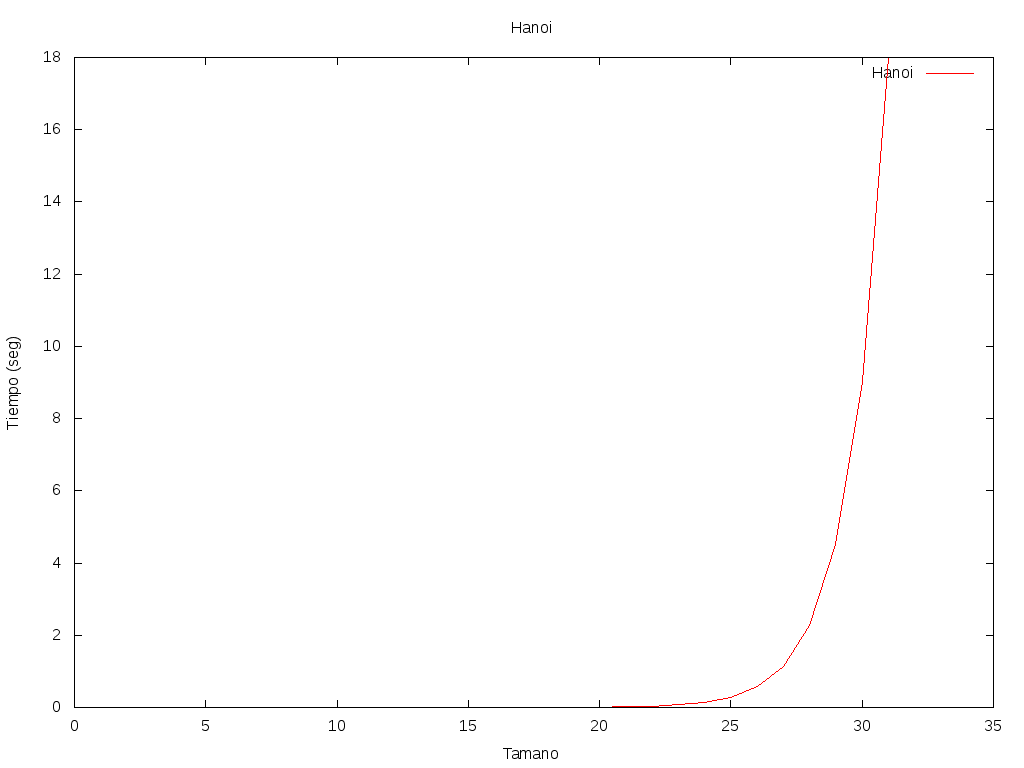
\includegraphics[width=0.7\linewidth]{imagenes/hanoiLines.png}
		\caption{Hanoi, gráfica empírica.}
		\label{fig:E19}
	\end{figure}
	
\end{frame}

\begin{frame}
	\frametitle{Hanoi}
	La gráfica híbrida obtenida ha sido:
	\begin{figure}
		\centering
		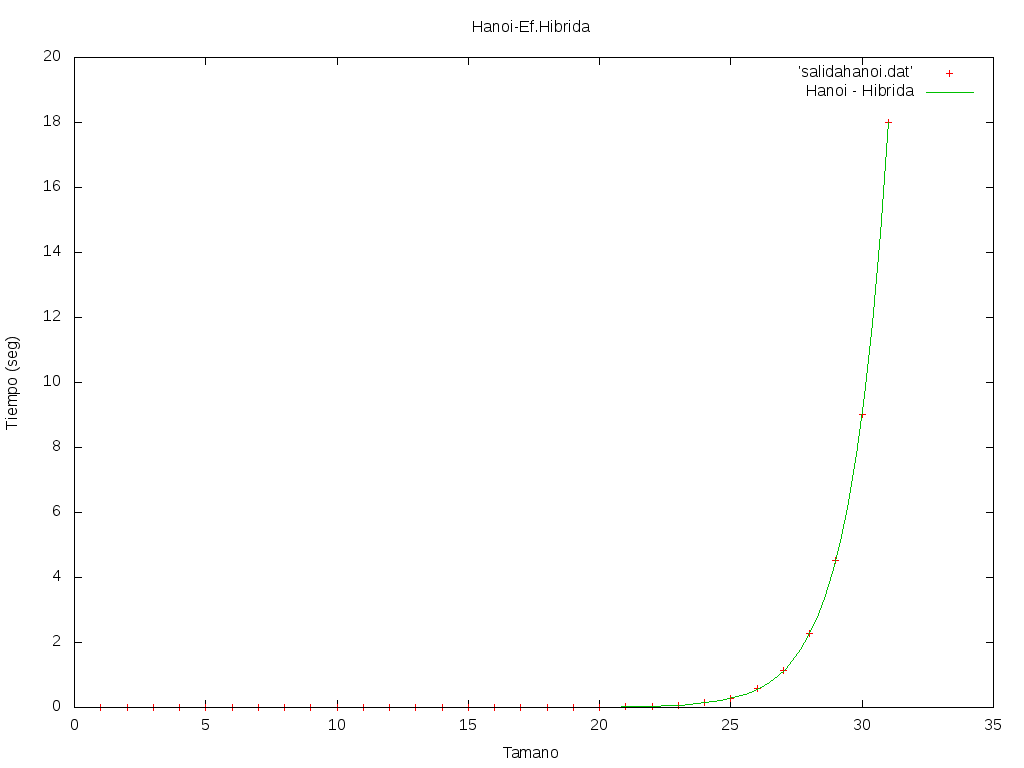
\includegraphics[width=0.7\linewidth]{imagenes/hanoi-hibrido.png}
		\caption{Hanoi, gráfica híbrida.}
		\label{fig:E20}
	\end{figure}
\end{frame}

\begin{frame}
	\frametitle{Hanoi}
	En este algoritmo hemos hecho varias comparaciones:
	\begin{itemize}
		\item Usando diferentes optimizaciones a la hora de compilar.
		\item Utilizando un lenguaje de programación distinto (Python vs C++).
	\end{itemize}
\end{frame}

\begin{frame}
	\frametitle{Hanoi en Python}
	La gráfica híbrida de la ejecución en Python frente a la ejecución en C++ es:
	\begin{figure}
		\centering
		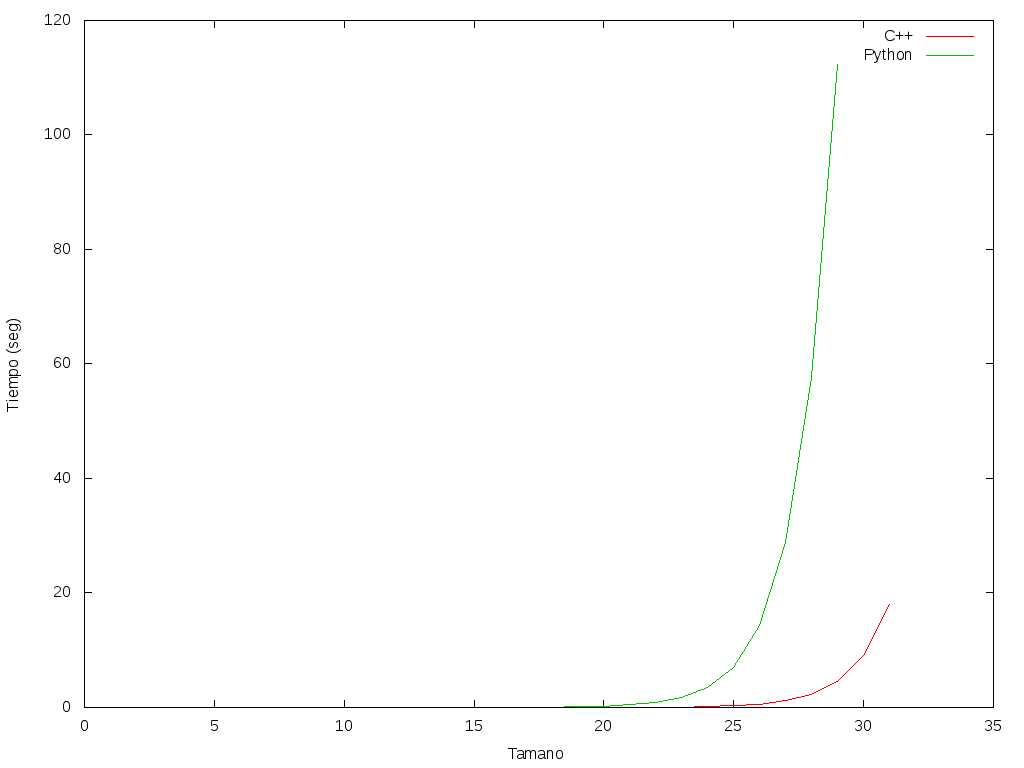
\includegraphics[width=0.7\linewidth]{imagenes/HanoiPy.png}
		\caption{Hanoi, Python - C++}
		\label{fig:E21}
	\end{figure}
\end{frame}

\begin{frame}
	\frametitle{Hanoi con diferentes optimizaciones}
	A continuación mostramos una gráfica con los tiempos del algoritmo en función de su optimización:
	\begin{figure}
		\centering
		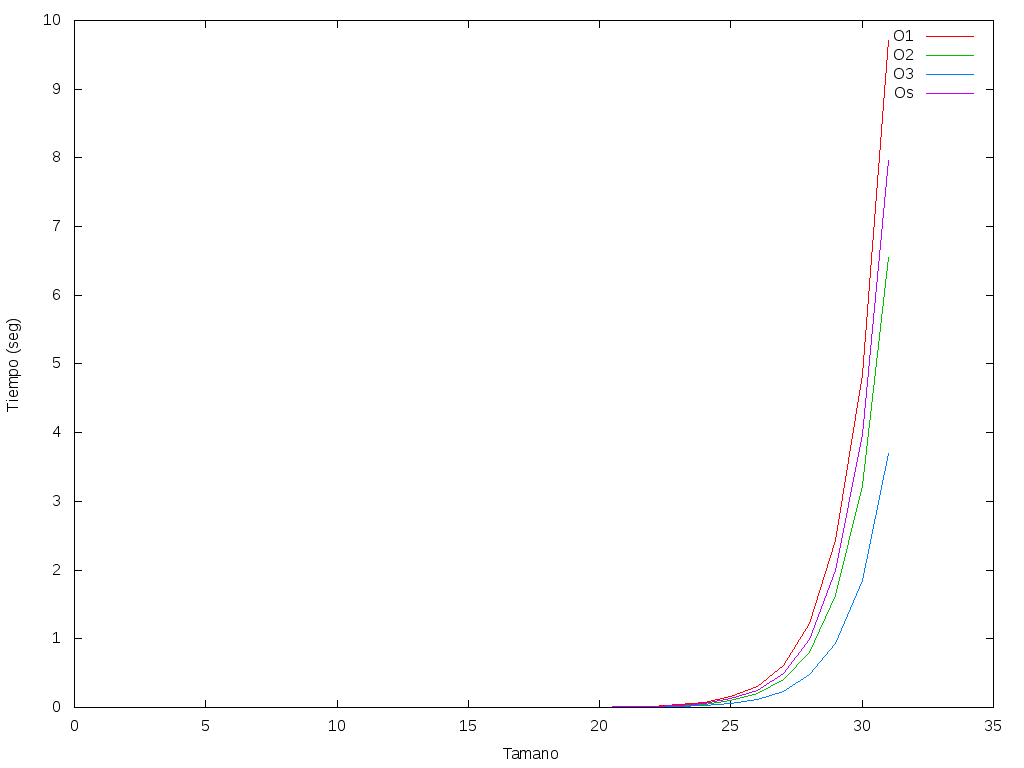
\includegraphics[width=0.7\linewidth]{imagenes/HanoiComparacion.png}
		\caption{Hanoi, gráfica con diferentes eficiencias.}
		\label{fig:E22}
	\end{figure}
\end{frame}

\begin{frame}
	\frametitle{Hanoi $O(2^n)$}
	Por último, mostramos el porcentaje de error así como las constantes ocultas.\\
	
	\begin{center}
		\begin{tabular}{| l | c | r |}
			\hline
			\textbf{Algoritmo} & \textbf{Constante Oculta} & \textbf{Error} \\ \hline
			Hanoi & a0 = 8.38461e-09 & +/- 3.095e-12    (0.03691\%)\\ \hline
		\end{tabular}
	\end{center}

\end{frame}



\begin{frame}
\Huge{\centerline{¿Preguntas?}}
\end{frame}

%----------------------------------------------------------------------------------------

\end{document} 